\section{Automatic I/O Activity Management Using Program Contexts}

%In developing \textsf{\small PCStream}, our key insight was that in most
%applications, (regardless of their I/O workload characteristics) a few dominant
%I/O activities exist and each dominant I/O activity   represents the
%application's important I/O context (e.g., for logging or for flushing).
%Furthermore, most dominant I/O activities tend to have distinct data lifetime
%patterns.  In order to distinguish data by their lifetimes, therefore, it is
%important to effectively distinguish dominant I/O activities from each other.
%For example, in update workloads, LBAs alone were effective in separating
%dominant I/O activities.  

{\color{blue}
In developing an automatic data lifetime predictor for general I/O workloads,
our key insight was that in most applications,}
the overall I/O behavior of 
applications is decided by a few dominant
I/O activities (e.g., logging and flushing). Moreover, 
data written by dominant I/O activities tend to have distinct lifetime patterns.
Therefore, if such dominant I/O activities of applications can be 
{\color{blue}
automatically detected and distinguished each other in an LBA-oblivious fashion, 
an automatic stream management technique can be developed for widely varying I/O workloads 
including append-only workloads.}
%(regardless of their I/O workload characteristics) a few dominant
%I/O activities exist and each dominant I/O activity   represents the
%application's important I/O context (e.g., for logging or for flushing).
%Furthermore, most dominant I/O activities tend to have distinct data lifetime
%patterns.  In order to distinguish data by their lifetimes, therefore, it is
%important to effectively distinguish dominant I/O activities from each other.
%For example, in update workloads, LBAs alone were effective in separating
%dominant I/O activities.  

In this paper, we argue that a program context (PC) can be
used to build an efficient general-purpose 
{\color{blue}classifier of dominant I/O activities with different data lifetimes.}
Here, a PC
represents an execution path of an application which invokes write-related
system call functions such as {\tt write()} and {\tt writev()}.  
There could be various ways of extracting PCs, 
but the most common approach~\cite{PC, PC2} is to
represent each PC with its PC ID which is computed by summing 
program counter values of all the functions along the execution path which
leads to a write() system call.

\begin{figure}[t]
%	\vspace{-10pt}
	\centering
	%\vspace{-8pt}
	\includegraphics[width=0.3\textwidth]{figure/writepath}
	\caption{An illustration of (simplified) execution paths of two dominant I/O activities in RocksDB.}
	\label{fig:iopath}
\end{figure}

%we represent the PC by summing program counter values of
%all the functions along the execution path which leads to a write system call.

\subsection{Program Context as a Unit of Lifetime Classification}
In order to illustrate that using PCs is an effective way to distinguish I/O
activities of an application and their data lifetime patterns, 
we measured data lifetime distributions of PCs from various applications with 
different I/O workloads.  
In this section, we report our evaluation results for three applications with distinct I/O
activities: RocksDB~\cite{RocksDB}, SQLite~\cite{SQLite}, and GCC~\cite{GCC}.
{\color{blue}
RocksDB shows the append-only workload while SQLite shows a workload 
that updates in place.
Both database workloads are expected to have distinct I/O activities 
for writing log files and data files.
GCC represents compile job that produdes many temporary files with several 
result files which may last longer.
}

In RocksDB, dominant I/O activities include logging, flushing and compaction.
Since these I/O activities are invoked through different 
function-call paths, so we can easily
identify dominant I/O activities of RocksDB using PCs.  
For example, Fig.~\ref{fig:iopath} shows 
(simplified) execution paths for 
logging and compaction in RocksDB and their PC ID values.  
The sum of program counter values of execution path
\texttt{WriteImpl()} $\rightarrow$ \texttt{WriteToWAL()} $\rightarrow$ \texttt{AddRecord()} is used
to represent a PC for the logging activity while  \texttt{Run()} $\rightarrow$
\texttt{ProcessKeyValueCompaction()} $\rightarrow$ \texttt{FinishCompactionFile()} is used
for compaction activity.

\begin{figure}[t]
\centering
\hfill
%\vspace{-10pt}
	\subfloat[Logging (manual)]{\includegraphics[width=0.2\textwidth]{figure/type_1}} % data from 4/03031953 
	\hspace{2pt}
	\subfloat[Logging (PC)]{\includegraphics[width=0.2\textwidth]{figure/pcID_2}}
\hfill
\vspace{7pt}
	\subfloat[Flushing (manual)] {\includegraphics[width=0.2\textwidth]{figure/type_3}}
	\hspace{2pt}
	\subfloat[Flushing (PC)]{\includegraphics[width=0.2\textwidth]{figure/pcID_3}}
%\vspace{-7pt}
\caption{Data lifetime distributions of different PCs for an append-only workload.} 
\label{fig:types_and_PCs}
%\vspace{-20pt}
\end{figure}


%\textcolor{red}{(TODO: 갑자기
%lifetime 이야기가 나옴. 없애도 큰 문제가 없을 듯...) \sout{Note that using a
%program context to distinguish data lifetimes is not new. For example, Ha {\it
%et al.} proposed a data separation technique based on the program
%context~\cite{PCHa}.  However, their work was neither designed for append-only
%workloads nor for modern multi-streamed SSDs.}}

To confirm our hypothesis that data lifetimes can be distinguished by tracking
dominant I/O activities and a PC is a useful unit of classification for 
different I/O activities,
we have conducted a set of experiments with RocksDB using two
different methods.  First, we manually identify dominant I/O activities by
inspecting the source code.  Second, we automatically detect dominant I/O
activities by extracting PCs for write-related system functions.
{\color{blue}
As expected, Fig.~\ref{fig:types_and_PCs} validates that dominant I/O activities 
show distinct data lifetime distributions over the logical address space.
For example, as shown in Figs.~\ref{fig:types_and_PCs}(a) and ~\ref{fig:types_and_PCs}(c), 
the logging activity and the flushing activity clearly exhibit quite different 
data lifetime distributions; while logging data have logging data have short lifetimes, 
data flushed by RocksDB are likely to have much longer lifetimes.
Furthermore, Figs.~\ref{fig:types_and_PCs}(b) and ~\ref{fig:types_and_PCs}(d) show that 
a PC-based lifetime separation technique produces the same lifetime 
classification accuracy as the manual technique. 
}

We have conducted additional experiments with SQLite and GCC which have
different I/O characteristics from RocksDB. In contrast to RocksDB that writes
almost all of the data in an append-only manner, SQLite 
writes most data in place while GCC write large data in an write-once mode.
Fig.~\ref{fig:updating_PCs} 
shows our experimental results for data lifetime distributions of the I/O
activities of SQLite and GCC.
As shown in Figs.~\ref{fig:updating_PCs}(a) and (b), the logging activity of
SQLite generates short-lived data.  This is because SQLite overwrites logging
data in a small and fixed storage space and then removes them soon.  We also
see that the logging activity is successfully identified by PCs. Similarly,
data lifetimes of temporary files generated by GCC are 
relatively short as shown in Figs.~\ref{fig:updating_PCs}(c) and ~\ref{fig:updating_PCs}(d) 
because of the write-once pattern of temporary files.
We observe that GCC
instances are forked and terminated, generating temporary files, but all those
activities are captured by PCs. 

\begin{figure}[t]
\centering
\hfill
%\vspace{-10pt}
	\subfloat[SQLite: logging (manual)]{\includegraphics[width=0.2\textwidth]{figure/sqlite_short_LBA_manual}} % data from py-tpcc/4/09151534
	\hspace{2pt}
	\subfloat[SQLite: logging (PC)]{\includegraphics[width=0.2\textwidth]{figure/sqlite_short_LBA}}
\hfill
\vspace{7pt}
	\subfloat[GCC: temp files (manual)] {\includegraphics[width=0.2\textwidth]{figure/compile_short_manual}} % data from 08231319
	\hspace{2pt}
	\subfloat[GCC: temp files (PC)]{\includegraphics[width=0.2\textwidth]{figure/compile_short_PC}}
%\vspace{-7pt}
\caption{Data lifetime distributions of different PCs for SQLite and GCC.} 
\label{fig:updating_PCs}
%\vspace{-20pt}
\end{figure}


\subsection{Extracting PCs}
A PC signature, which is used as a unique ID of each program context,
is defined
to be the sum of program counters along the execution path of function calls
that finally reaches a write-related system function.  In theory, program
counter values in the execution path can be extracted in a relatively
straightforward manner.  Except for inline functions, every function call
involves pushing the address of the next instruction of a caller as a return
address to the stack, followed by pushing a frame pointer value.  By referring
to frame pointers, we are able to back-track stack frames of a process and
selectively get return addresses for generating a PC signature.
For example, Fig.~\ref{fig:getpc}(a) illustrates a stack of RocksDB corresponding
to Fig.~\ref{fig:iopath}, where return addresses are pushed before calling
the \textsf{\small  write()}, \textsf{\small AddRecord()} and \textsf{\small
WriteToWAL()} functions.  Since frame pointer values in the stack hold the
addresses of previous frame pointers, we can easily obtain return addresses and
accumulate them to compute a PC signature.  

%For example,
%Fig.~\ref{fig:getpc}(a) shows abstracted execution paths of log data and
%compaction data in RocksDB.  The return addresses are pushed before calling the
%\textsf{\small  write()}, \textsf{\small AddRecord()} and \textsf{\small
%WriteToWAL()} functions.  Fig.~\ref{fig:getpc}(b) illustrates how a PC
%signature is obtained by back-tracking the stack.  Since frame pointer values
%in the stack hold the addresses of previous frame pointers, we can easily
%obtain return addresses and accumulate them to compute a PC signature.  

The frame pointer-based approach for computing a PC signature, however, is not
always possible because modern C/C++ compilers often do not use a frame pointer
for improving the efficiency of register allocation.  One example is a {\tt
-fomit-frame-pointer} option of GCC~\cite{GCC}.  This option enables to use a frame
pointer as a general-purpose register for performance, but makes it difficult for us
to back-track return addresses along the call chains.  

\begin{figure}[t]
%	\vspace{-10pt}
	\centering
	%\vspace{-8pt}
	%\subfloat[Abstracted execution paths of two I/O activities of RocksDB.]{\includegraphics[width=0.3\textwidth]{figure/writepath}}  
	%\vspace{-14pt}
	%\hfill
	\subfloat[with the frame pointer.]{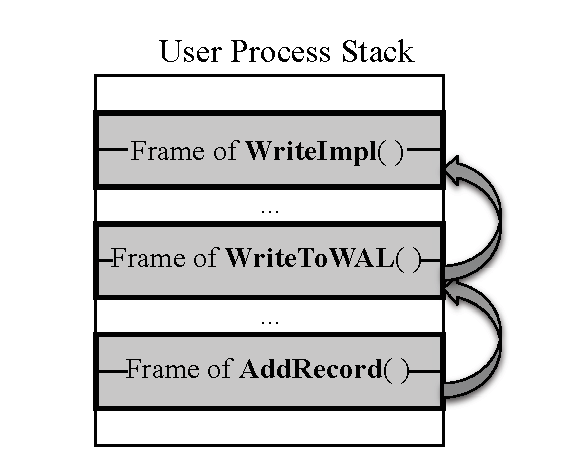
\includegraphics[width=0.15\textwidth]{figure/getpc1}}
	\subfloat[without the frame pointer.]{\includegraphics[width=0.22\textwidth]{figure/getpc2}}
	%\vspace{-9pt}
	\caption{The examples of PC extraction methods.}
	%\caption{An example execution path and its PC extraction.} %shane part
	\label{fig:getpc}
	%\vspace{-20pt}
\end{figure}

We employ a simple but effective workaround for back-tracking a call stack when
a frame pointer is not available.  When a write system call is made,
we scan every word in the stack
and checks if it belongs to process's code segment.  If the scanned stack word
holds a value within the address range of the code segment, it assumes that it
is a return address.  Since scanning the entire stack may takes too long, we stop
the scanning step once a sufficient number of return address candidates are found.
In the current implementation, the scanning process stops early once 
five return address candidates are identified.  
Even though it is quite ad-hoc, this restricted scan is quite effective
in distinguishing different PCs because it is very unlikely that two different PCs
reach the same write() system call through the same execution subpath 
that covers five proceeding function calls. 
In our evaluation on a PC with 3.4 GHz Intel CPU, the overhead of the
restricted scan was almost negligible, taking only 300$\sim$400 $n$sec per
\textsf{\small write()} system call.

